\subsection{GraphBLAST GraphBLAS}


GraphBLAST~\cite{Yang:2019:GBL} is the first high-performance GPU (graphics processing unit) implementation of GraphBLAS. Inspired by the design of GBTL, the architecture of GraphBLAST is also C++ based and maintains a separation of concerns between a top-level interface defined by the GraphBLAS C API specification and the low-level backend. 

One novel aspect about GraphBLAST is that it supports performance-oriented optimizations such as direction-optimization (also known as push-pull traversal), which was discovered by Beamer, Asanovic and Patterson~\cite{Beamer:2012:DOB} and generalized by Shun~\cite{Shun:2013:Ligra} to other graph algorithms. Yang, Bulu\c{c} and Owens~\cite{Yang:2018:IPE} show that this optimization is key for a GraphBLAS implementation to meet the performance of state-of-the-art graph frameworks on the GPU like Gunrock~\cite{Wang:2017:GGG}. In each iteration of an \verb'GrB_mxv', the GraphBLAST backend checks whether the vector sparsity was has crossed a threshold $k$. If it has gone above the threshold, then the traversal will switch from push to pull. If it has gone below the threshold, then the traversal will switch from pull to push. If neither outcome has occurred, then it will use the traversal it used in a previous iteration. 

To support direction-optimization, the GraphBLAST backend maintains a SparseVector and DenseVector object as shown in Figure~\ref{fig:graphblast}. The push traversal is performed using Gustavson's method as a sparse-matrix sparse-vector multiply (SpMSpV) between the SparseVector and the adjacency matrix transpose in CSC format. The pull traversal is performed in a dot-product manner as a sparse-matrix dense-vector multiply (SpMV) between the DenseVector and the adjacency matrix in CSR format. This raises the issue of having to keep around two copies of each \verb'GrB_Matrix' object when it is not symmetric. An environmental variable is used to control whether the user wants this performance-oriented storage, or whether they want a more memory-inexpensive storage of only CSR or only CSC in which case the direction-optimization feature is disabled.

\begin{figure}[t]
	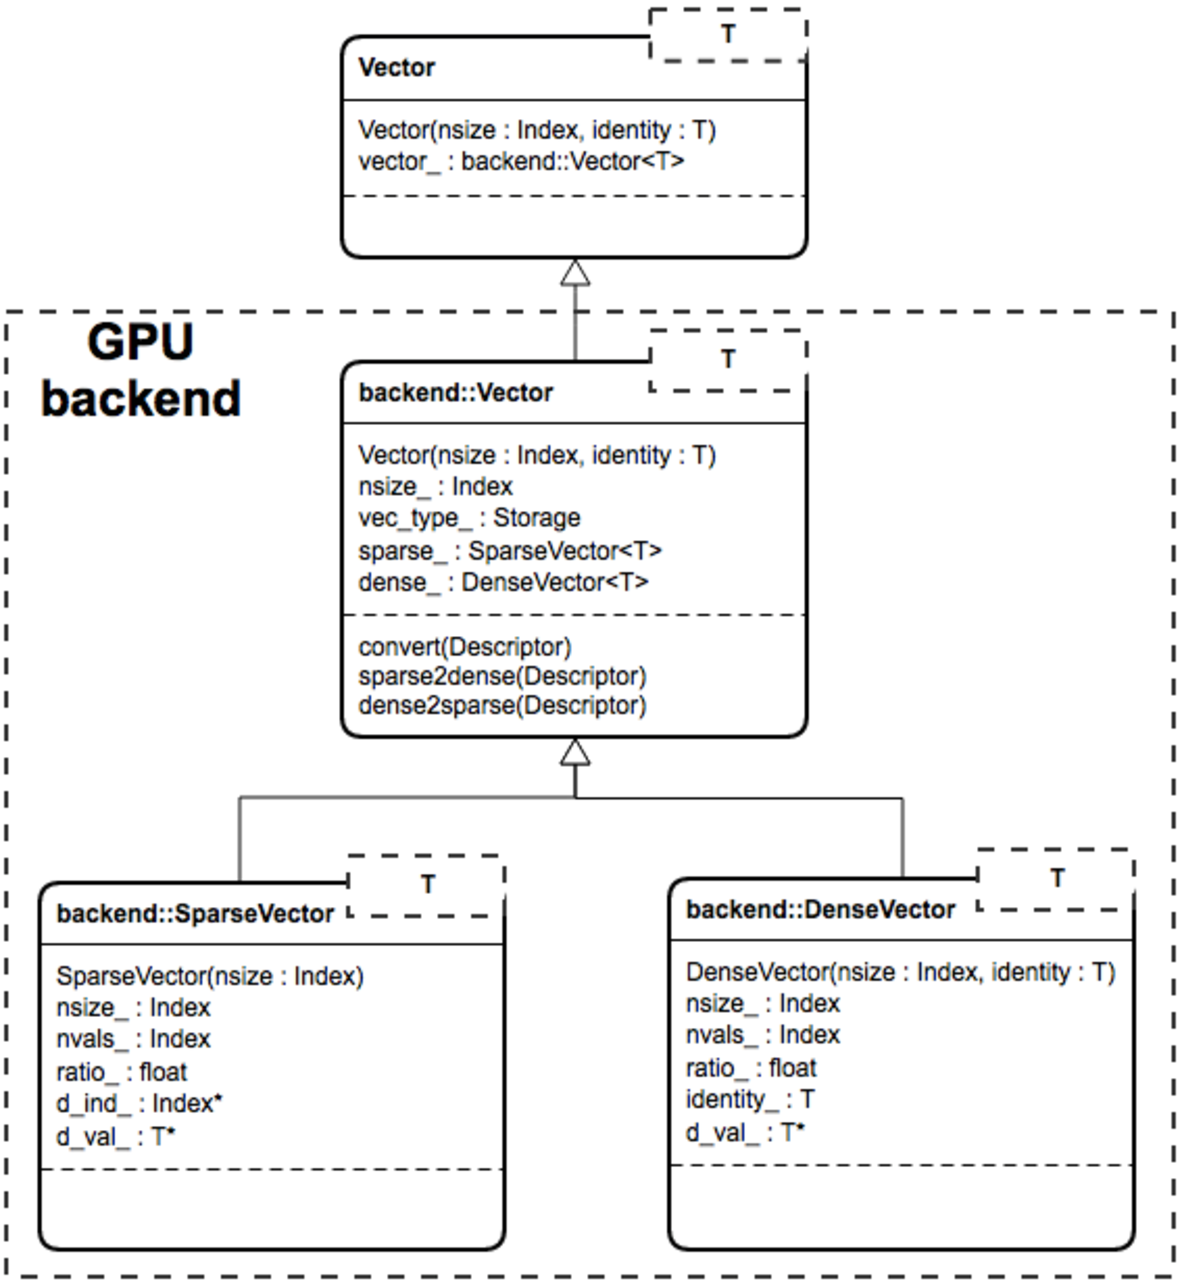
\includegraphics[width=\linewidth]{fig/graphblast}
	\caption{\textbf{GraphBLAST Vector UML diagram.}\label{fig:graphblast}}
\end{figure}

Direction-optimization is a good example where the power of abstracting away implementation details shines through, and the linear algebraic approach to graph analytics is at its most powerful. The end user has two conflicting desires:

\begin{enumerate}
	\item They want to communicate their request \emph{abstractly} enough that they do not have to decide whether the matrix-vector multiply is implemented as push, pull or any of the myriad possible ways.
	\item They want their computation to be described \emph{specifically} enough that the computer can optimize for the best approach for doing the computation.
\end{enumerate}

This desire is met by \verb'GrB_mxv', which is at the same time \emph{abstract} enough to not limit the computer in choosing push traversal when it should be choosing pull traversal, yet \emph{specific} enough that the computer has enough information to cut corners and pick the best algorithm.

Table~\ref{tab:loc} shows a comparison of how many lines of code it takes an implementation of GraphBLAS to express a given algorithm in C++. It is compared with two state-of-the-art graph frameworks in shared memory, the aforementioned Ligra~\cite{Shun:2013:Ligra} and GraphIt~\cite{Zhang:2018:GHP}, which is a DSL (domain specific language) designed for expressing graph algorithms.

\begin{table}[t]
	\centering
	\begin{tabular}{lccc}
		\toprule
		Algorithm      & Ligra~\cite{Shun:2013:Ligra} & GraphIt~\cite{Zhang:2018:GHP} & GraphBLAS  \\ \midrule
		Breadth-first-search & 29 & 22  & 25 \\
		Single-source shortest-path   & 55 & 25 & 25 \\
		Local graph clustering  & 84 & N/A  & 45 \\ \bottomrule
	\end{tabular}
	\caption{Comparison of lines of C++ application code counted by `cloc' except for numbers of GraphIt, which come from the paper~\cite{Zhang:2018:GHP}. N/A means not implemented. The specific GraphBLAS implementation for this comparison is GraphBLAST~\cite{Yang:2019:GBL}.\label{tab:loc}}
		%\vspace{-2em}
\hrule
\end{table}
